
\documentclass{homework}
\course{Math 5522H}
\author{Alex Li}
\usepackage{amsmath}
\DeclareMathOperator{\Mat}{Mat}
\DeclareMathOperator{\End}{End}
\DeclareMathOperator{\Hom}{Hom}
\DeclareMathOperator{\id}{id}
\DeclareMathOperator{\image}{im}
\DeclareMathOperator{\rank}{rank}
\DeclareMathOperator{\nullity}{nullity}
\DeclareMathOperator{\trace}{tr}
\DeclareMathOperator{\Spec}{Spec}
\DeclareMathOperator{\Sym}{Sym}
\DeclareMathOperator{\pf}{pf}
\DeclareMathOperator{\Ortho}{O}
\DeclareMathOperator{\diam}{diam}
\DeclareMathOperator{\Real}{Re}
\DeclareMathOperator{\Imag}{Im}
\DeclareMathOperator{\Arg}{Arg}
\DeclareMathOperator{\Log}{Log}

\newcommand{\C}{\mathbb{C}}
\newcommand{\R}{\mathbb{R}}
\newcommand{\Z}{\mathbb{Z}}
\newcommand{\N}{\mathbb{N}}


\DeclareMathOperator{\sla}{\mathfrak{sl}}
\newcommand{\norm}[1]{\left\lVert#1\right\rVert}
\newcommand{\transpose}{\intercal}

\newcommand{\conj}[1]{\overline{#1}}
\newcommand{\abs}[1]{\left|#1\right|}

%%% My commands, for solutions %%%

\usepackage{amssymb}
\usepackage{xifthen}
\usepackage{listings}
\usepackage{tikz} % Guide http://bit.ly/gNfVn9
\usetikzlibrary{decorations.markings}
\DeclareMathOperator{\Res}{Res}

% To write df/(dx), use \pfrac{f}{x}
\newcommand{\pfrac}[2]{\frac{\partial #1}{\partial #2}}
% Partial derivative. To take d^2f/(dxdy), use \ppfrac[y]{f}{x}
% To take d^2f/(dx^2), use ppfrac{f}{x}
\newcommand{\ppfrac}[3][]{\frac{\partial^2 #2}{\ifthenelse{\isempty{#1}}{\partial #3^2}{\partial #3\partial #1}}}
\newcommand{\oo}[0]{\infty}

 \newenvironment{solution}
   {\renewcommand\qedsymbol{$\blacksquare$}\begin{proof}[Solution]}
     {\end{proof}}
       
       % Code listing environment  
       \lstnewenvironment{code}{\lstset{basicstyle=\ttfamily, mathescape=true, breaklines=true}}{}

       % When you want to see how many pages your HW is
       \usepackage{lastpage}
       \usepackage{fancyhdr}
       \pagestyle{fancy} 
       \cfoot{\thepage\ of \pageref{LastPage}}




\begin{document}
\maketitle

\begin{inspiration}
Some of the most important results (e.g. Cauchy's theorem) are so surprising at first sight that nothing short of a proof can make them credible.
\byline{Sir Harold Jeffreys} % and where is this quotation from?
\end{inspiration}

\section{Terminology}

\begin{problem}
  What is a \textbf{Jordan curve}?
  \end{problem}
  \begin{solution}
  A Jordan curve is a simple closed piecewise smooth function $\gamma:[a,b]\mapsto \C$.
  \end{solution}
  \begin{problem}
    Define the \textbf{winding number} $n(\gamma,z)$ of a piecewise
      smooth closed curve $\gamma$ around a point $z \in \C$.
      \end{problem}
      \begin{solution}
      It's the net number of times you spin around clockwise, or
      \[n(\gamma, z) = \frac{1}{2\pi i}\int_\gamma \frac{1}{x-z}dx \]

      \end{solution}
      \section{Numericals}

      \begin{problem}\label{Fresnel integral}
      Compute the \textbf{Fresnel integrals}
        \[
            \int_0^\infty \sin \left( x^2 \right) \, dx \mbox{ and } \int_0^\infty \cos \left( x^2 \right) \, dx.
              \]
              \end{problem}
              We can do them both at once, let $f(x) = \cos(x^2) + i\sin(x^2)$. Then the real part of $\int_0^\infty f(x)dx$ is the value of the cosine integral, and the imaginary part is the value of the sin integral. Noting that $f(x) = e^{ix^2}$, we itegrate around the eighth circle of radius $R$, $\gamma$ in figure \ref{octant-tikz}. 

              \begin{figure}[h]
              \begin{tikzpicture}
              \draw [<->] (-4, 0) -- (4, 0);
              \draw [<->] (0, -4) -- (0, 4);
              \node [below] at (4.24, 0) {$R$};
              \node [right] at (3, 3) {$\theta=\pi/4$};
              \begin{scope}[very thick,decoration={
                  markings,
                      mark=at position 0.5 with {\arrow{>}}}
                          ] 
                          \draw[postaction={decorate}] (0,0) -- (4.24, 0);
                          \draw[postaction={decorate}] (3,3) -- (0,0);
                          \draw[postaction={decorate}] (4.24, 0) arc [radius=4.24, start angle=0, end angle=45];
                          \end{scope}
                          \end{tikzpicture}
                          \caption{The curve $\gamma$ for \ref{Fresnel integral}}
                          \label{octant-tikz}
                          \end{figure}
                          \begin{align*}
                          \int_\gamma e^{iz^2}
                          &= \int_0^R e^{iz^2}dz + \int_0^{\frac{\pi}{4}} (ie^{i\theta}) e^{i(Re^{i\theta})^2} d\theta + \int_0^R e^{5\pi/4}e^{i(ze^{i\pi/4})^2)}dz \\
                          &= \int_0^R e^{iz^2}dz + \int_0^{\frac{\pi}{4}} ie^{iR^2\cos(2\theta) - R^2\sin(2\theta) + i\theta} d\theta - e^{\pi/4} \int_0^R e^{-z^2}dz
                          \end{align*}
                          Letting $R$ go to infinity, the middle term vanishes since the real part of the exponent $R^2\sin(2\theta) + \cos(\theta)$ goes to $-\infty$. The last term becomes the classic statistics integral with value $\frac{\sqrt{\pi}}{2}$. Since $\int_\gamma f(x)$ is the integral of a holomorphic function around a closed curve, by cauchy's theorem it's value is 0 so we can deduce that 
                          \[\int_0^\infty e^{iz^2}dz = e^{\pi/4} \int_0^R e^{-z^2}dz =  \frac{1+i}{\sqrt{2}}\frac{\sqrt{\pi}}{2} = \frac{\sqrt{\pi}}{\sqrt{8}} + \frac{i\sqrt{\pi}}{\sqrt{8}}\]
                          so 
                            \[
                                \int_0^\infty \sin \left( x^2 \right) \, dx = \int_0^\infty \cos \left( x^2 \right) \, dx = \frac{\sqrt{\pi}}{\sqrt{8}}
                                  \]
                                  \begin{problem}
                                    For an integrable function $f : \R \to \C$, define the
                                      \textbf{Fourier transform} of $f$, denoted $\hat{f}$, by
                                        \[
                                            {\hat {f}}(\xi ) := \int _{-\infty }^{\infty} f(x) \, e^{-2\pi ix \xi} \,dx.
                                              \]
                                                Find the Fourier transform of $f(x) = e^{-\pi x^2}$.
                                                \end{problem}
                                                \begin{solution}
                                                We solve this by completing the square in the exponent:
                                                \begin{align}\label{completed_square_fourier}
                                                -\pi x^2 - 2\pi ix\xi = -\pi(x-i\xi)^2 - \pi \xi^2
                                                \end{align}
                                                We want to do something like below,
                                                \begin{align*}
                                                {\hat {f}}(\xi ) &=  \int _{-\infty }^{\infty} e^{-\pi x^2 -2\pi ix \xi} \,dx\\
                                                &=  e^{-\xi^2\pi}\int _{-\infty }^{\infty} e^{-\pi (x-i\xi)^2} \,dx\quad \color{purple} \text{ By Eq. \ref{completed_square_fourier}}
                                                \end{align*}
                                                This integral can almost be evaluated with a $u$ subsitution of 
                                                \[u = x-i\xi.\]
                                                However, the bounds of integration will be messed up and we will be going over the complex numbers. So let's consider the closed rectangular contour that goes on a straight line between the four points below.
                                                \[R \mapsto R - i\zeta \mapsto - R - i\zeta \mapsto -R\]
                                                As $R\to\infty$, the sides of this rectangle with nonzero imaginary derivative will disappear as
                                                \[
                                                \abs{\int_{-\zeta}^{0} e^{-\pi((\pm R+ix) -i\zeta)^2} dx} \leq \abs{\zeta} \abs{e^{-\pi R}}\to 0.
                                                \]
                                                Thus the integral of the bottom of the rectangle is equal to the integral going backwards along the top of the rectangle, which we can compute
                                                \begin{align*}
                                                \hat f(\zeta) &=  e^{-\xi^2\pi}\int_{-\infty}^\infty e^{-\pi x^2} \,dx\\
                                                &=  \frac{e^{-\xi^2\pi}}{\sqrt{\pi}}\int_{-\infty}^\infty e^{-x^2} \,dx\quad \color{purple} u = \sqrt{\pi}x, du = \sqrt{\pi} dx\\
                                                &=  \frac{e^{-\xi^2\pi}}{\sqrt{\pi}} \sqrt{\pi} =  e^{-\xi^2\pi}
                                                \end{align*}

                                                \end{solution}
                                                \section{Exploration}

                                                \begin{problem}\label{conjz_no_primitive}
                                                  Does the function $f : \C \to \C$ given by $f(z) = \conj{z}$ have a
                                                    primitive?
                                                    \end{problem}
                                                    \begin{solution}
                                                    Let $F$ be a primitive for $f$ and $\gamma: [0,1]\mapsto \C$ with $\gamma(t)=e^{it2\pi}$ be a closed curve.
                                                    Then
                                                    \begin{align*}
                                                        0 = F(\gamma(2\pi)) - F(\gamma(0)) = \int_\gamma \conj{z} = \int_\gamma \frac{1}{z} = 2\pi i,
                                                        \end{align*}
                                                        a contradiction.
                                                        \end{solution}
                                                        \begin{problem}
                                                          We proved Goursat's theorem for rectangles.  Without simply
                                                            recapitalulating the proof (e.g., your argument should not again
                                                              invoke \ref{nested-subsets-convergence}), deduce a theorem for
                                                                \textit{triangles} from our result about rectangles.
                                                                \end{problem}
                                                                \begin{solution}
                                                                We will prove the following:
                                                                \begin{theorem}\label{triangle-theorem}
                                                                Let $\gamma_{\Delta}$ be a curve around some triangle be a triangle contained in an open set $S$, and $f:S\mapsto \C$ be holomorphic. Then
                                                                \[\int_{\gamma_{\Delta}} f = 0\]
                                                                In fact, this generalizes to any polygon with no holes in it whose interior is contained in $S$ (by gluing positively oriented triangles together to make that polygon and cancelling).
                                                                \end{theorem}
                                                                Choose some side of the triangle as well as a small $\delta$. Now, draw a rectangle parallel to that side of height $\delta$ as wide as possible, and then draw a rectangle on that and so on until you can't anymore. (See Figure \ref{curve-triangle-rectangles}). 
                                                                \begin{figure}[h]
                                                                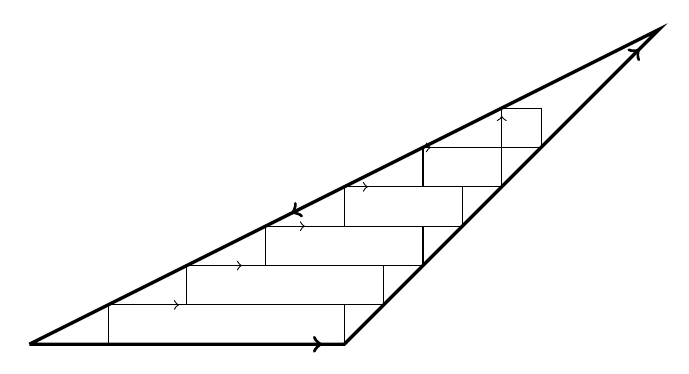
\begin{tikzpicture}
                                                                \begin{scope}[very thick,decoration={
                                                                    markings,
                                                                        mark=at position 0.2 with {\arrow{>}},
                                                                            mark=at position 0.5 with {\arrow{>}},
                                                                                mark=at position 0.8 with {\arrow{>}}}
                                                                                    ] 
                                                                                    \draw[postaction={decorate}] (0,0) -- (4, 0) -- (8, 4) -- (0,0);
                                                                                    \end{scope}
                                                                                    \begin{scope}[decoration={
                                                                                        markings,
                                                                                            mark=at position 0.2 with {\arrow{>}}}
                                                                                                ]
                                                                                                \draw[postaction={decorate}] (1, 0) -- (1, .5) -- (4, .5) -- (4, 0) -- (1, 0);
                                                                                                \draw[postaction={decorate}] (2, .5) -- (2, 1) -- (4.5, 1) -- (4.5, .5) -- (2, .5);
                                                                                                \draw[postaction={decorate}] (3, 1) -- (3, 1.5) -- (5, 1.5) -- (5, 1) -- (3, 1);
                                                                                                \draw[postaction={decorate}] (4, 1.5) -- (4, 2) -- (5.5, 2) -- (5.5, 1.5) -- (4, 1.5);
                                                                                                \draw[postaction={decorate}] (5, 2) -- (5, 2.5) -- (6, 2.5) -- (6, 2) -- (5, 2);
                                                                                                \draw[postaction={decorate}] (6, 2.5) -- (6, 3) -- (6.5, 3) -- (6.5, 2.5) -- (6, 2.5);
                                                                                                \end{scope}
                                                                                                \end{tikzpicture}
                                                                                                \caption{Cutting a triangle into small rectangles}
                                                                                                \label{curve-triangle-rectangles}
                                                                                                \end{figure}
                                                                                                Since each of the rectangles have a value of 0, the integral around the triangle is equal to the sum of the integrals around the smaller triangles between the thin rectangles and the big triangle.

                                                                                                Now, because $f$ is continous on the compact set that is the interior of $\gamma_{\Delta}$ it is uniformly continuous, so we can choose $\delta$ such that the value of $f$ varies by less than $\epsilon$ at any two points on the same small cut up piece. As the pieces get smaller, the top strangely shaped piece will have a very small arc length and so the value of the integral around it goes to 0, so we can ignore it. Next we can bound the integral around any other triangle $\gamma_{i}$. If $f$ is a constant, then the integral around the triangle is 0, so
                                                                                                \[\abs{\int_{\gamma_i} f dz} = \abs{\int_{\gamma_i} f dz- \inf_{\gamma_i}(f)} \leq |\gamma_i|\epsilon\].

                                                                                                Now, any given small triangle has it's longest side as part of the contour $\gamma_{\Delta}$, so the sum of the perimeters of all of the triangles is bounded above by $3\abs{\gamma_{\Delta}}$. Thus we can bound the integral around $\gamma_\Delta$ by choosing $\delta$ so as to make $\epsilon$ tiny:
                                                                                                \[\abs{\int_{\gamma_\Delta} f}\leq 3\abs{\gamma_{\Delta}}\epsilon\to 0\]
                                                                                                \end{solution}

                                                                                                \begin{problem}
                                                                                                  Suppose $f, g : \C \to \C$ are holomorphic and agree on the unit
                                                                                                    circle.  How do $f$ and $g$ relate?  Morally, this problem is
                                                                                                      related to \ref{identity-theorem}.
                                                                                                      \end{problem}
                                                                                                      \begin{solution}
                                                                                                      Let's consider $f-g$, it's holomorphic and equal to 0 on the unit circle. Call the positively oriented curve going around the unit circle $\gamma$. By Cauchy's Integral formula, 
                                                                                                      \[(f-g)(z) = \frac{1}{2\pi i}\int_{\gamma}\frac{(f-g)(w)}{z-w}dw\]
                                                                                                      And this is $0$ since the numerator is $0$.
                                                                                                      \end{solution}

                                                                                                       \begin{problem}
                                                                                                          Suppose $f : \C \to \C$ is holomorphic, and consider the circle
                                                                                                             $\gamma$ with center $z_0$.  How does the real part of the average
                                                                                                                value of $f$ on the circle $\gamma$ relate to $f(z_0)$?
                                                                                                                 \end{problem}
                                                                                                                 \begin{solution}
                                                                                                                 By Cauchy's integral formula, 
                                                                                                                 \begin{align*}
                                                                                                                 f(z_0) &= \frac{1}{2\pi i}\int_{\gamma} \frac{f(z)}{z_0 - z}dz\\
                                                                                                                 &= \frac{1}{2\pi i}\int_{0}^{2\pi} \frac{f(z_0 + e^{it})}{e^{it}}ie^{it} dz\\
                                                                                                                 &= \frac{1}{2\pi}\int_{0}^{2\pi} f(z_0 + e^{it}) dz
                                                                                                                 \end{align*}
                                                                                                                 And this last expression is the average value of $f$ on the circle $\gamma$, so $f(z_0)$ is is equal to average value of $f$ on the circle $\gamma$.

                                                                                                                 \end{solution}
                                                                                                                  \begin{problem}
                                                                                                                     Recalling \ref{harmonic-conjugate}, suppose $u, v : \C \to \R$ are
                                                                                                                        harmonic functions and $f = u + iv$ is holomorphic, so $u$ and $v$
                                                                                                                           are harmonic conjugates.  Find the \textbf{Poisson kernel} for the
                                                                                                                              unit disc, i.e., find a function $P_r(\theta)$ so that
                                                                                                                                 \[
                                                                                                                                      u(re^{i\theta}) = \frac {1}{2\pi} \int_{-\pi }^{\pi } P_{r}(\theta -t) \, u(e^{it}) \, dt
                                                                                                                                         \]
                                                                                                                                            for $r < 1$.
                                                                                                                                             \end{problem}
                                                                                                                                             \begin{solution}
                                                                                                                                             We can recover the value at $re^{i\theta}$ by an integral of $u$ over the unit circle using Cauchy's integral formula
                                                                                                                                             \begin{align*}
                                                                                                                                             u(re^{i\theta}) &= \frac{1}{2\pi i}\int_{\gamma} \frac{u(e^{it})}{re^{i\theta} - e^{it}}\\
                                                                                                                                             &= \frac{1}{2\pi i}\int_{-\pi}^{\pi} \frac{u(e^{it})ie^{it}}{re^{i\theta} - e^{it}}\\
                                                                                                                                             &= \frac{1}{2\pi}\int_{-\pi}^{\pi} \frac{u(e^{it})}{re^{i(\theta - t)} - 1}\\
                                                                                                                                             \end{align*}
                                                                                                                                             Thus 
                                                                                                                                             \[P_r(\theta) = \frac{1}{re^{i\theta} - 1}\]
                                                                                                                                             is the Poisson kernel.

                                                                                                                                             \end{solution}
                                                                                                                                             \section{Prove or Disprove and Salvage if Possible}

                                                                                                                                             \begin{problem}
                                                                                                                                               Suppose $D = \{ z \in \C : \abs{z} < 1 \}$ and $f : D \to \C$ is
                                                                                                                                                 continuous and $\gamma : [a,b] \to D$ is a piecewise smooth curve.
                                                                                                                                                   Then $\displaystyle\int_\gamma f\, dz = 0$.
                                                                                                                                                   \end{problem}
                                                                                                                                                    \begin{solution}
                                                                                                                                                     No, let $f(x)=1$ and $\gamma$ be any non-closed curve. Even if it's closed, if $f$ is not holomorphic, then going around a rectangle may be a problem (for example consider the computation in \ref{conjz_no_primitive}). So we really want to suppose that $\gamma$ is closed and $f$ is holomorphic. We will prove the following.
                                                                                                                                                     \begin{theorem}\label{general-curve-theorem}
                                                                                                                                                     Let $\gamma$ be a piecewise smooth curve in an open set $S$, and $f:S\mapsto \C$ be holomorphic. If the interior of $\gamma$ is contained in $S$, then \[\int_{\gamma} fdz = 0\].
                                                                                                                                                     \end{theorem}
                                                                                                                                                     Theorem \ref{triangle-theorem} tells use this is true if $\gamma$ is the curve of a polygon. Since $\gamma$ is smooth, it is rectifiable, so we can draw a polygonal path $\gamma(t_0), \gamma(t_1), \dots, \gamma(t_{n-1}), \gamma(t_n)$ with $\gamma(t_n)=\gamma(t_0)$ that approximates $\gamma$. Since $S$ is open we can ensure this path in contained inside of it. By rectifiablity, we can choose the path such that for any $\delta > 0$,
                                                                                                                                                     \[\sum_{i=0}^{n-1}\abs{\gamma(t_i) - \gamma(t_{i+1})} - \int_{t_i}^{t_{i+1}} f(\gamma(t)) dt \leq \delta \]
                                                                                                                                                     Let $\gamma_{i}'$ be the integral on the line directly from $t_i$ to $t_{i+1}$ and then back from $t_{i+1}$ to $t_{i}$ along the curve $\gamma$. We can choose $t_i$ to be close enough to each other that any two points on $\gamma_{i}'$ are at most $\delta$ away from each other, and since the polygon is compact and $f$ is continuous, for any $\epsilon > 0$ we can choose $\delta$ such that 
                                                                                                                                                     \[x - y < \delta \implies f(x) - f(y) < \epsilon\].

                                                                                                                                                     Now, since the line integral of interior of the polygon is 0 by Theorem \ref{triangle-theorem}, the value of the line integral around $\gamma$ is bounded by the sum of the integrals of the segments between the approximating polygon and the curve. Then
                                                                                                                                                     \begin{align*}
                                                                                                                                                     \abs{\int_{\gamma} fdz} &\leq \sum_{i=0}^{n-1}\abs{\int_{\gamma_{i}'} f dt}\\
                                                                                                                                                     &= \sum_{i=0}^{n-1}\abs{\int_{\gamma_{i}'} f - \inf_{\gamma_{i}'}f dt}\color{purple}\text{ closed line integral of constant is 0}\\
                                                                                                                                                     &\leq \sum_{i=0}^{n-1}\abs{\gamma_{i}'}(\sup_{\gamma_{i}'}f - \inf_{\gamma_{i}'}f)  dt\\
                                                                                                                                                     &\leq \sum_{i=0}^{n-1}\abs{\gamma_{i}'}\epsilon dt\\
                                                                                                                                                     &\leq \epsilon((2\int_{\gamma(t)}dt +\delta)\to 0
                                                                                                                                                     \end{align*}    
                                                                                                                                                     Thus the line integral around $\gamma$ is 0.
                                                                                                                                                      \end{solution} 
                                                                                                                                                       
                                                                                                                                                       \begin{problem}
                                                                                                                                                         Suppose $U$ is an open set and $f : U \to \C$ is analytic and
                                                                                                                                                           $\gamma : [a,b] \to U$ is a piecewise smooth curve.  Then
                                                                                                                                                             $\displaystyle\int_\gamma f \, dz = 0$.
                                                                                                                                                             \end{problem}
                                                                                                                                                             \begin{solution}
                                                                                                                                                             False- again, $\gamma$ must be closed, and the interior of $\gamma$ should be contained in $U$. In this case we can apply \ref{general-curve-theorem}.
                                                                                                                                                             Otherwise a counter-example can be given by noting that $1/z$ is defined on the open set $\C/\{0\}$. For $\gamma$ the unit circle, $\int_\gamma 1/z=2\pi i\neq 0$.
                                                                                                                                                             \end{solution}


                                                                                                                                                             \begin{problem}
                                                                                                                                                               Define $\gamma_r : [0,2\pi] \to \C$ by
                                                                                                                                                                 $\gamma_r(\theta) = r e^{i \theta}$, and for real numbers
                                                                                                                                                                   $R > r > 0$, define the annulus
                                                                                                                                                                     \[
                                                                                                                                                                         A(r,R) := \{ z \in \C : r < |z| < R \}
                                                                                                                                                                           \]
                                                                                                                                                                             and suppose $f : A(r/2,2R) \to \C$ is holomorphic.  Then
                                                                                                                                                                               \[
                                                                                                                                                                                   \int_{\gamma_r} f \, dz = \int_{\gamma_R} f \, dz.
                                                                                                                                                                                     \]
                                                                                                                                                                                     \end{problem}
                                                                                                                                                                                     \begin{solution}
                                                                                                                                                                                     True. Consider integrating along the 2 curves in Fig. \ref{annulus-curve}. The two curves are closed and can be compressed to a point along the holomorphic region, so the integral along them both is 0. The two horizontal lines will cancel out, so we have the claim.
                                                                                                                                                                                     \begin{figure}[h]
                                                                                                                                                                                     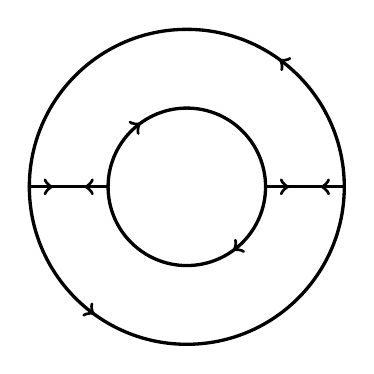
\begin{tikzpicture}
                                                                                                                                                                                     \begin{scope}[very thick,decoration={
                                                                                                                                                                                         markings,
                                                                                                                                                                                             mark=at position 0.3 with {\arrow{>}}}
                                                                                                                                                                                                 ] 
                                                                                                                                                                                                 \draw[postaction={decorate}] (-1, 0) arc [radius=1, start angle=180, end angle=0];
                                                                                                                                                                                                 \draw[postaction={decorate}] (2, 0) arc [radius=2, start angle=0, end angle=180];
                                                                                                                                                                                                 \draw[postaction={decorate}] (-2, 0) arc [radius=2, start angle=180, end angle=360];
                                                                                                                                                                                                 \draw[postaction={decorate}] (1, 0) arc [radius=1, start angle=360, end angle=180];
                                                                                                                                                                                                 \draw[postaction={decorate}] (1,0) -- (2,0);
                                                                                                                                                                                                 \draw[postaction={decorate}] (2,0) -- (1,0);
                                                                                                                                                                                                 \draw[postaction={decorate}] (-1,0) -- (-2,0);
                                                                                                                                                                                                 \draw[postaction={decorate}] (-2,0) -- (-1,0);
                                                                                                                                                                                                 \end{scope}
                                                                                                                                                                                                 \end{tikzpicture}
                                                                                                                                                                                                 \caption{Annulus Curves, one is on the top half and the other is on the bottom half.}
                                                                                                                                                                                                 \label{annulus-curve}
                                                                                                                                                                                                 \end{figure}
                                                                                                                                                                                                 \end{solution}
                                                                                                                                                                                                 \pagebreak
                                                                                                                                                                                                 \begin{problem}\label{cauchy-integral-formula}
                                                                                                                                                                                                 Define $B_R(0) := \{ z \in C : \abs{z} < R \}$ and suppose
                                                                                                                                                                                                   $f : B_R(0) \to \C$ is holomorphic and let $\gamma$ be the
                                                                                                                                                                                                     positively-oriented circle of positive radius $r < R$.  Then
                                                                                                                                                                                                       \[
                                                                                                                                                                                                           f(a) = \int_\gamma \frac{f(z)}{z-a} \, dz.
                                                                                                                                                                                                             \]
                                                                                                                                                                                                               and moreover
                                                                                                                                                                                                                 \[
                                                                                                                                                                                                                     f'(a) = \int_\gamma \frac{f(z)}{(z-a)^2} \, dz.
                                                                                                                                                                                                                       \]  
                                                                                                                                                                                                                       \end{problem}
                                                                                                                                                                                                                       \begin{solution}
                                                                                                                                                                                                                       This is true up to a factor of $2\pi i$ for any $a$ in the interior of $\gamma$. For the first claim,
                                                                                                                                                                                                                       \begin{align*}
                                                                                                                                                                                                                       \int_\gamma \frac{f(z)}{z-a}dz &= \int_\gamma \frac{f(z) - f(a)}{z-a}dz + f(a)\int_\gamma \frac{1}{z-a}dz
                                                                                                                                                                                                                       \end{align*}
                                                                                                                                                                                                                       The rightmost integral is the integral of $\frac{1}{z}$ around a circle containing the origin shifted by $a$, so it is $2\pi i$.
                                                                                                                                                                                                                       \begin{align}
                                                                                                                                                                                                                       \label{cauchys-integral-formula-really}
                                                                                                                                                                                                                       \int_\gamma \frac{f(z)}{z-a}dz &= \int_\gamma \frac{f(z) - f(a)}{z-a}dz + f(a)2\pi i
                                                                                                                                                                                                                       \end{align}
                                                                                                                                                                                                                       Now, we can draw a super small circle of radius $\delta$ around $a$ contained in $B_R(0)$. Splitting this circle up into 2 curves in the spirit of the image \ref{annulus-curve}, and noting that the two curves have line integral 0, we see that the integral around $B_R(0)$ is equivalent to the integral around the small circle centered at $a$. Letting $\delta$ go to 0, 
                                                                                                                                                                                                                       \begin{align*}
                                                                                                                                                                                                                       \lim_{\delta\to 0} \int_{\gamma_{\delta}} \frac{f(z)-f(a)}{z-a} dz &= \lim_{\delta\to 0} \int_{\gamma_{\delta}} \frac{f(a+h)-f(a)}{h} dz \color{purple}\quad |h| = \delta\\
                                                                                                                                                                                                                       &\leq \frac{|2\gamma_{\delta}|}{\delta}\sup{f(a+h) - f(a)}\\
                                                                                                                                                                                                                       &\leq \frac{2\pi\delta}{\delta}\epsilon \leq 0 
                                                                                                                                                                                                                       \end{align*}
                                                                                                                                                                                                                       Here we can use the continuity of $f$ to ensure that we can choose a $\delta$ such that $a+h - a<\delta \implies f(a+h) - f(a) < \epsilon$. Thus by Eq. \ref{cauchys-integral-formula-really}
                                                                                                                                                                                                                       \begin{align}\label{cauchys-integral-formula-clean}
                                                                                                                                                                                                                       \frac{1}{2\pi i}\int_\gamma \frac{f(z)}{z-a}dz &= f(a)
                                                                                                                                                                                                                       \end{align}
                                                                                                                                                                                                                       For the second equation, let's take the derivative of both sides with respect to $a$ with the quotient rule
                                                                                                                                                                                                                       \begin{align}\label{cauchys-integral-formula-clean-d}
                                                                                                                                                                                                                       \frac{1}{2\pi i}\int_\gamma \frac{f(z)}{(z-a)^2}dz &= f'(a)
                                                                                                                                                                                                                       \end{align}
                                                                                                                                                                                                                       \end{solution}

                                                                                                                                                                                                                       \begin{problem}\label{cauchy-inequalities}If $f : U \to \C$ is
                                                                                                                                                                                                                         holomorphic and $U \supset B_r(z_0)$, then
                                                                                                                                                                                                                           \[
                                                                                                                                                                                                                                \abs{f(z_0)} \leq \sup_{z \in \partial B_r(z_0)} \abs{f(z)}
                                                                                                                                                                                                                                   \]
                                                                                                                                                                                                                                      and
                                                                                                                                                                                                                                         \[
                                                                                                                                                                                                                                              \abs{f'(z_0)} \leq \sup_{z \in \partial B_r(z_0)} \abs{f(z)}. % missing (1/r) factor
                                                                                                                                                                                                                                                 \]
                                                                                                                                                                                                                                                  \end{problem}
                                                                                                                                                                                                                                                   \begin{solution}
                                                                                                                                                                                                                                                   WLOG let $z_0=0.$ By Eq. \ref{cauchys-integral-formula-clean},
                                                                                                                                                                                                                                                   \begin{align*}
                                                                                                                                                                                                                                                   f(0) &= \frac{1}{2\pi i}\int_0^{2\pi} \frac{f(re^{it})ire^{it}}{re^{it}}dt\\
                                                                                                                                                                                                                                                   &= \frac{1}{2\pi}\int_0^{2\pi} f(re^{it}) dt
                                                                                                                                                                                                                                                   \end{align*}
                                                                                                                                                                                                                                                   So $f(0)$ is the average value on the boundary, and thus $\abs{f(z_0)} \leq \displaystyle\sup_{z \in \partial B_r(z_0)} |f(z)|$.
                                                                                                                                                                                                                                                   By Eq. \ref{cauchys-integral-formula-clean-d},
                                                                                                                                                                                                                                                   \begin{align*}
                                                                                                                                                                                                                                                   \abs{f'(0)} &= \abs{\frac{1}{2\pi i}\int_0^{2\pi} \frac{f(re^{it})ire^{it}}{(re^{it})^2}dt}\\
                                                                                                                                                                                                                                                   &\leq \frac{1}{2\pi r}\int_0^{2\pi} \frac{\abs{f(re^{it})}}{\abs{e^{it}}} dt\\
                                                                                                                                                                                                                                                   &\leq \frac{1}{r}\left(\frac{1}{2\pi}\int_0^{2\pi} \abs{f(re^{it})} dt\right)
                                                                                                                                                                                                                                                   \end{align*}
                                                                                                                                                                                                                                                   Thus 
                                                                                                                                                                                                                                                   \begin{align}\label{derivative-dies-holomorphic}
                                                                                                                                                                                                                                                   \abs{f'(z_0)} \leq \frac{1}{r}\displaystyle\sup_{z \in \partial B_r(z_0)} |f(z)|
                                                                                                                                                                                                                                                   \end{align}
                                                                                                                                                                                                                                                    \end{solution}

                                                                                                                                                                                                                                                    \begin{problem}\label{liouville-theorem}Recall that a function $f : U \to \C$ is
                                                                                                                                                                                                                                                      \textbf{bounded} if there exists $M > 0$ so that for all $z \in U$
                                                                                                                                                                                                                                                        we have $\abs{f(z)} \leq M$.  A bounded holomorphic function
                                                                                                                                                                                                                                                          $f : U \to \C$ is constant.
                                                                                                                                                                                                                                                          \end{problem}
                                                                                                                                                                                                                                                          \begin{solution}
                                                                                                                                                                                                                                                          False, consider $f:B_1(0)\mapsto \C, f(z) = z$. This is bounded, since $\abs{f(z)}\leq 1$. But it's clearly not constant. However, we can prove it if we take $U=\C$.

                                                                                                                                                                                                                                                          Choose a point $z_0$, and construct a ball of a massive radius $r$ around it. Then by \ref{derivative-dies-holomorphic}, 
                                                                                                                                                                                                                                                          \[\abs{f'(z_0)} \leq \frac{1}{r}\sup_{z \in \partial B_r(z_0)} \abs{f(z)} \leq rM \to 0\]
                                                                                                                                                                                                                                                          Thus the derivative of $f$ is 0 everywhere, so $f$ is constant.
                                                                                                                                                                                                                                                          \end{solution}
                                                                                                                                                                                                                                                          \begin{problem}
                                                                                                                                                                                                                                                            For every polynomial $p \in \C[z]$ there is $z \in \C$ so that $p(z) = 0$.
                                                                                                                                                                                                                                                            \end{problem}
                                                                                                                                                                                                                                                            \begin{proof}
                                                                                                                                                                                                                                                            False. Consider the polynomial $p(z)=1$. Instead we prove the following:
                                                                                                                                                                                                                                                            \begin{theorem}
                                                                                                                                                                                                                                                            If a polynomial $p \in \C[z]$ has no zeros, it is constant.
                                                                                                                                                                                                                                                            \end{theorem}
                                                                                                                                                                                                                                                            \[
                                                                                                                                                                                                                                                            \abs{p(z)} = \abs{\sum_{n=0}^d a_nz^n} \geq \abs{z}^d - \sum_{n=0}^{d-1} \abs{a_n}\abs{z}^n
                                                                                                                                                                                                                                                            \]
                                                                                                                                                                                                                                                            Once $\abs{z}$ gets sufficently big (say $\abs{z}>M$), the leading term will dominate and we can say that, for some $M_2$ $\abs{p(z)}>M_2$.

                                                                                                                                                                                                                                                            Suppose that $p(z)$ never takes on the value $0$. Then $\frac{1}{p(z)}$ is holomorphic, and outside of the ball of radius $M$, it's value is at most $\frac{1}{M_2}$. And it's holomorphic hence continuous and thus also bounded inside the compact set that is the ball of radius $M$. Thus $\frac{1}{p(z)}$ is bounded, and by \ref{liouville-theorem}, it is constant.
                                                                                                                                                                                                                                                            \end{proof}
                                                                                                                                                                                                                                                            \end{document}
